\section{Sitios web con herramienta de software y datos recolectados}
Aquí, se presentan enlaces a los sitios web específicos donde se puede acceder a la herramienta de software mejorada desarrollada durante el proyecto, así como a los conjuntos de datos recolectados a lo largo de la investigación. Este recurso facilita a los lectores y colaboradores la exploración directa de la herramienta y la revisión de los datos utilizados en el estudio, brindando una visión integral y accesible de los resultados y contribuciones generadas.

\begin{itemize}
    \item GitHub: \url{https://github.com/pat19218/Tesis_2023}
    \item Banco de datos: \href{https://drive.google.com/drive/u/1/folders/1aTNy2e-KkGNi9qVemx3-I05KnxCGLlTQ}{Drive}
\end{itemize}

\section{Pruebas con algoritmo VAT}
En la sección dedicada a las pruebas con el algoritmo VAT, se llevó a cabo un exhaustivo análisis de las características de las señales bioeléctricas en distintos dominios: frecuencia, tiempo y wavelets. Cada prueba se diseñó para evaluar la capacidad del algoritmo VAT en la identificación de tendencias de agrupamiento bajo variadas condiciones. Con el propósito de estudiar el impacto de la cantidad de épocas empleadas en el proceso, se realizaron pruebas sucesivas, incrementando gradualmente este parámetro. Este enfoque sistemático permitió una evaluación detallada de la efectividad del algoritmo en la visualización y discernimiento de patrones de agrupamiento en las señales, brindando perspectivas valiosas sobre su rendimiento en diferentes contextos y condiciones.

\subsection{VAT características en el dominio de frecuencia}
Se exploraron detalladamente los resultados obtenidos al aplicar este algoritmo para la visualización de patrones de agrupamiento en las señales bioeléctricas. La representación gráfica generada por el VAT, donde se distinguen los grupos a través de la variación de colores, proporciona una visión integral de la estructura de los datos. Aunque se observa cierta diferenciación entre los grupos, la distinción no es tan pronunciada, lo cual plantea un escenario interesante en términos de la complejidad de los patrones presentes en las señales. Esta característica, aunque implica un mayor desafío en la identificación visual de los grupos, puede brindar \textit{insights} valiosos sobre la naturaleza sutil de las relaciones entre las señales, destacando la importancia de técnicas adicionales para una interpretación más precisa y detallada como se observan en las Figuras~\ref{vat: vat_freq_100} - \ref{vat: vat_freq_2700}.

\begin{figure}[H]
	\centering
	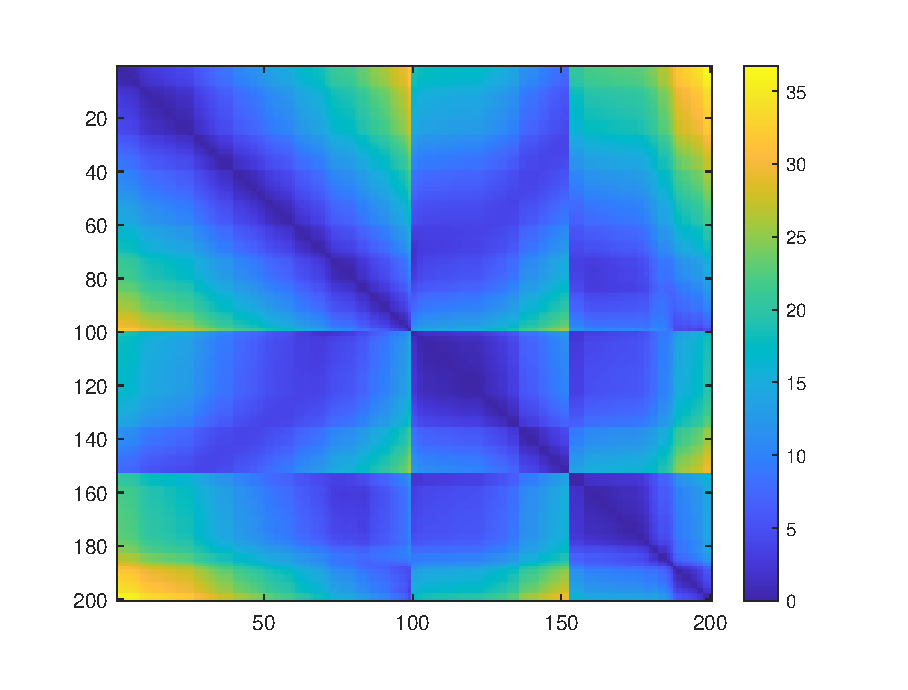
\includegraphics[width=0.85\textwidth]{figuras/vat_freq_100.eps}
	\caption{VAT usando 100 épocas de características tipo frecuencia.}
	\label{vat: vat_freq_100}
\end{figure}
\begin{figure}[H]
	\centering
	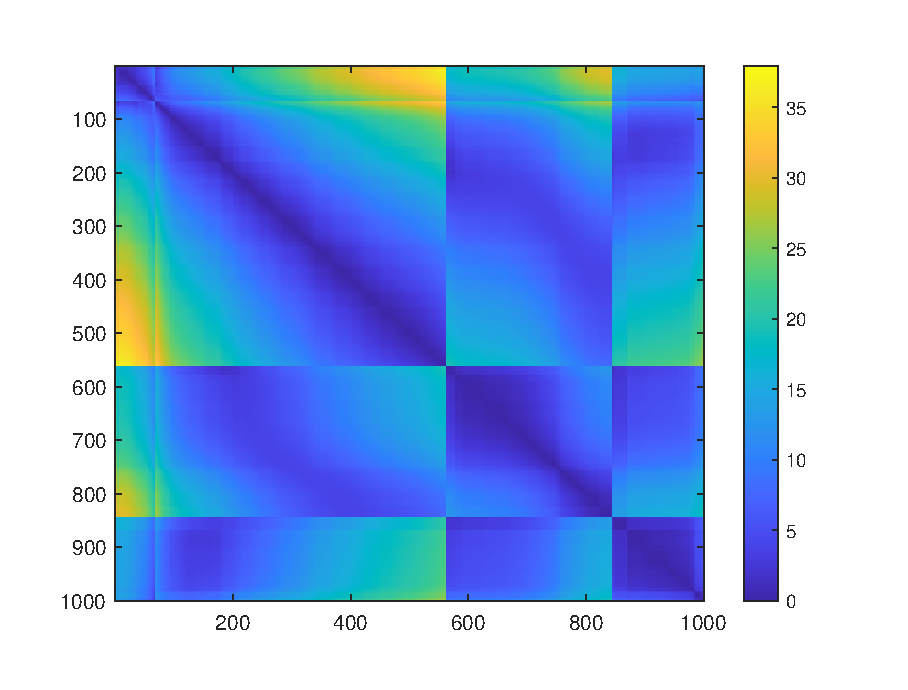
\includegraphics[width=0.85\textwidth]{figuras/vat_freq_500.eps}
	\caption{VAT usando 500épocas de características tipo frecuencia.}
	\label{vat: vat_freq_500}
\end{figure}
\begin{figure}[H]
	\centering
	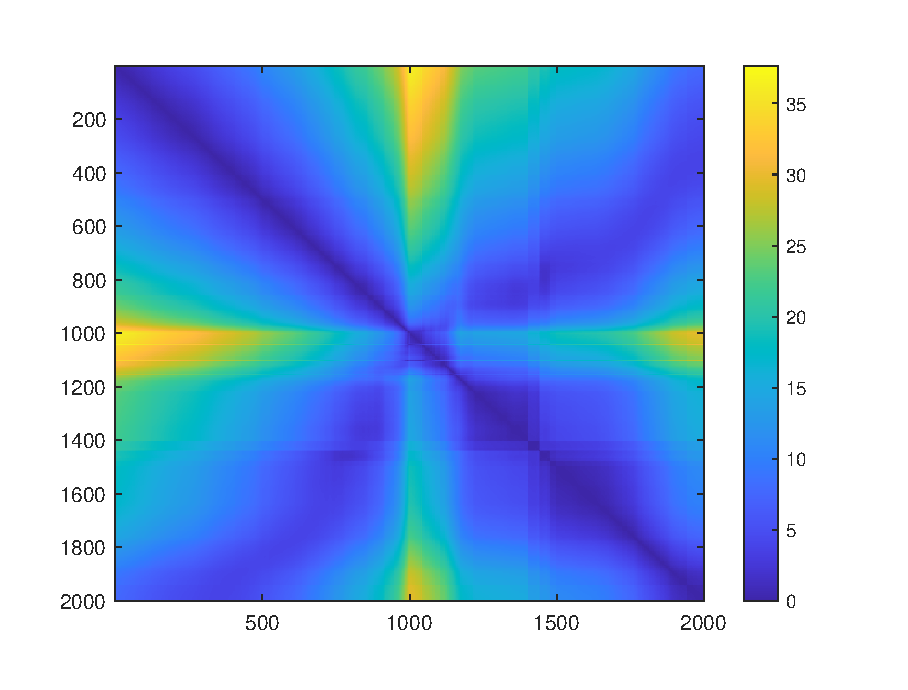
\includegraphics[width=0.85\textwidth]{figuras/vat_freq_1000.eps}
	\caption{VAT usando 1000 épocas de características tipo frecuencia.}
	\label{vat: vat_freq_1000}
\end{figure}
\begin{figure}[H]
	\centering
	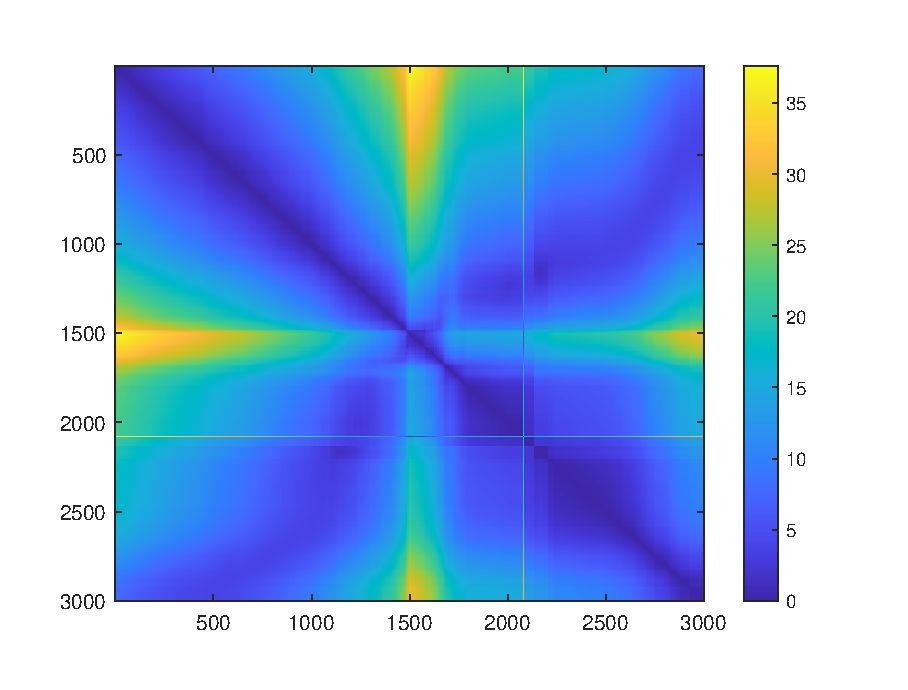
\includegraphics[width=0.85\textwidth]{figuras/vat_freq_1500.eps}
	\caption{VAT usando 1500 épocas de características tipo frecuencia.}
	\label{vat: vat_freq_1500}
\end{figure}
\begin{figure}[H]
	\centering
	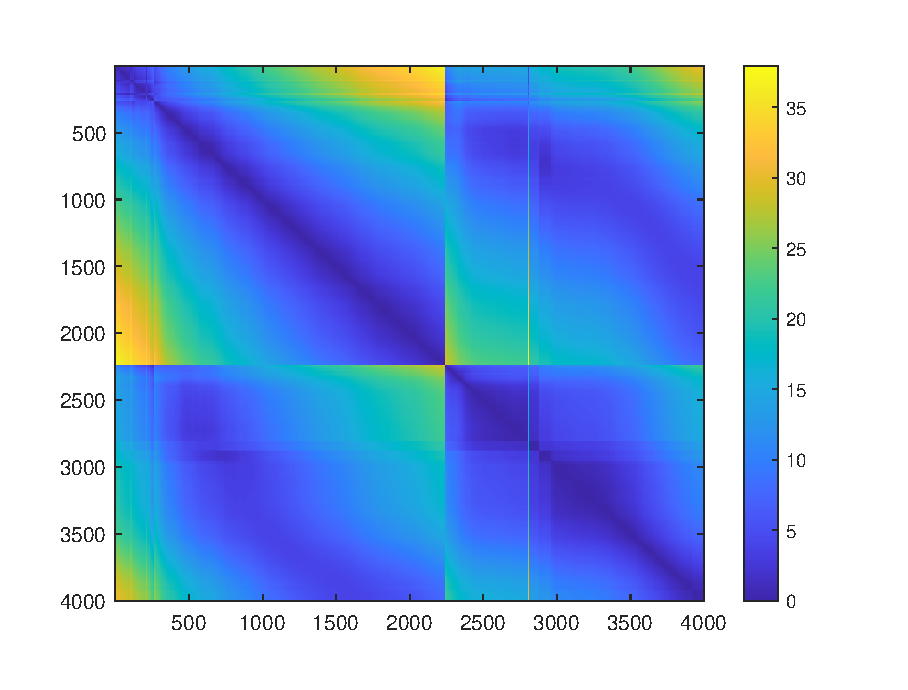
\includegraphics[width=0.85\textwidth]{figuras/vat_freq_2000.eps}
	\caption{VAT usando 2000 épocas de características tipo frecuencia.}
	\label{vat: vat_freq_2000}
\end{figure}
\begin{figure}[H]
\centering
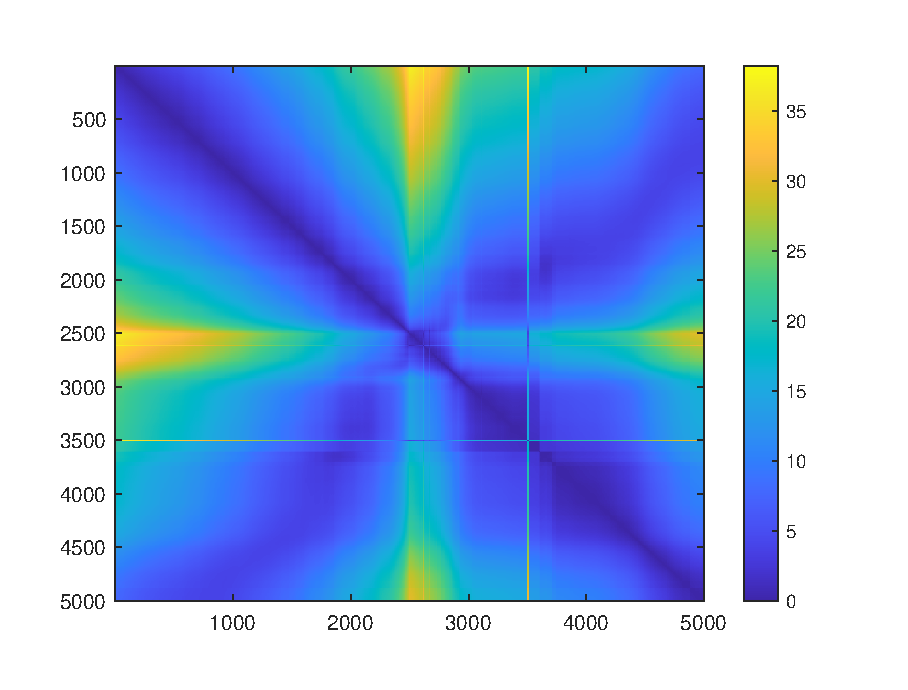
\includegraphics[width=0.85\textwidth]{figuras/vat_freq_2500.eps}
\caption{VAT usando 2500 épocas de características tipo frecuencia.}
\label{vat: vat_freq_2500}
\end{figure}
\begin{figure}[H]
	\centering
	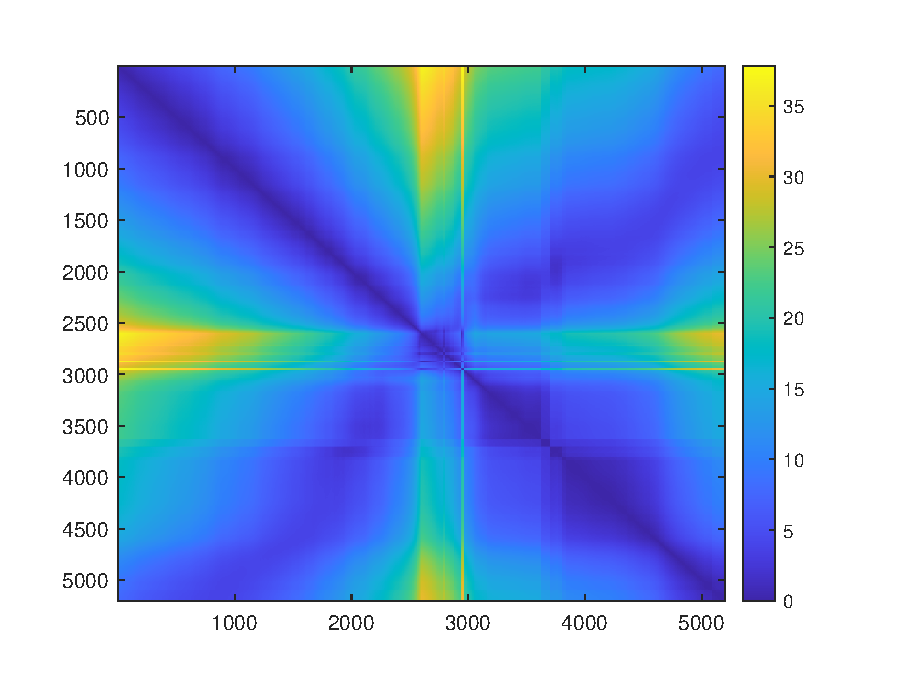
\includegraphics[width=0.85\textwidth]{figuras/vat_freq_2600.eps}
	\caption{VAT usando 2600 épocas de características tipo frecuencia.}
	\label{vat: vat_freq_2600}
\end{figure}
\begin{figure}[H]
	\centering
	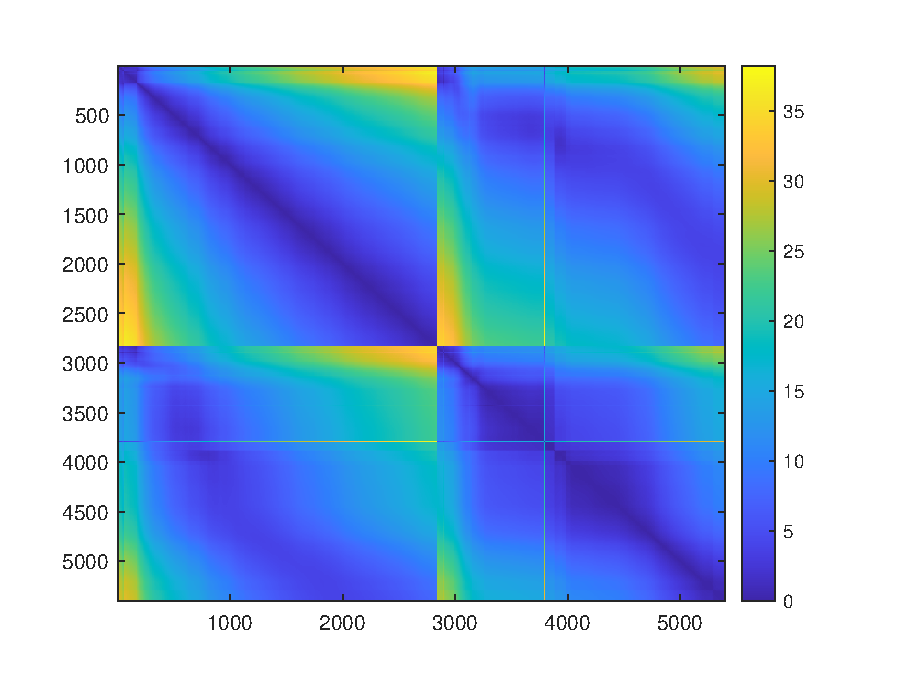
\includegraphics[width=0.85\textwidth]{figuras/vat_freq_2700.eps}
	\caption{VAT usando 2700 épocas de características tipo frecuencia.}
	\label{vat: vat_freq_2700}
\end{figure}

\subsection{VAT características en el dominio de tiempo continuo}
En la exploración de las características en el dominio del tiempo continuo mediante la aplicación del algoritmo VAT, se observa una distribución particular de los datos. La representación visual destaca por la ausencia de una clara diferenciación de grupos, ya que la variación de colores revela una proximidad significativa entre todos los puntos de datos. Esta cercanía en la representación visual sugiere que las características analizadas en este contexto particular pueden no ser tan discriminatorias como se esperaba para identificar patrones distintivos de agrupamiento.Este hallazgo insta a una reflexión más profunda sobre la naturaleza de las características consideradas y la exploración de enfoques alternativos para la identificación de patrones en el dominio del tiempo continuo, como se observa en las Figuras~\ref{vat: vat_time_100} - \ref{vat: vat_time_2300}. 

\begin{figure}[H]
	\centering
	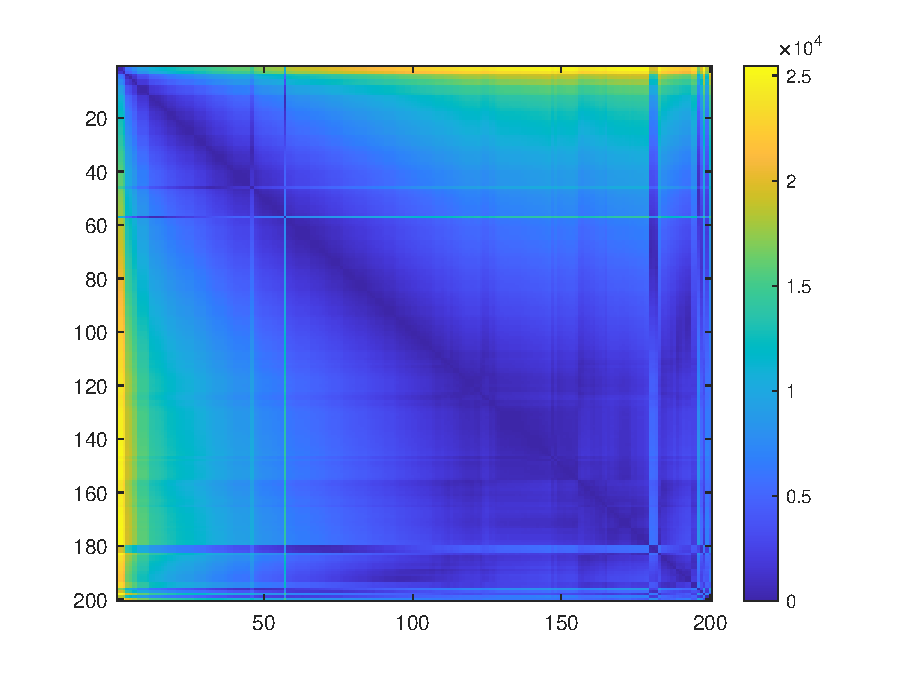
\includegraphics[width=0.85\textwidth]{figuras/vat_time_100.eps}
	\caption{VAT usando 100 épocas de características tipo tiempo continuo.}
	\label{vat: vat_time_100}
\end{figure}
\begin{figure}[H]
	\centering
	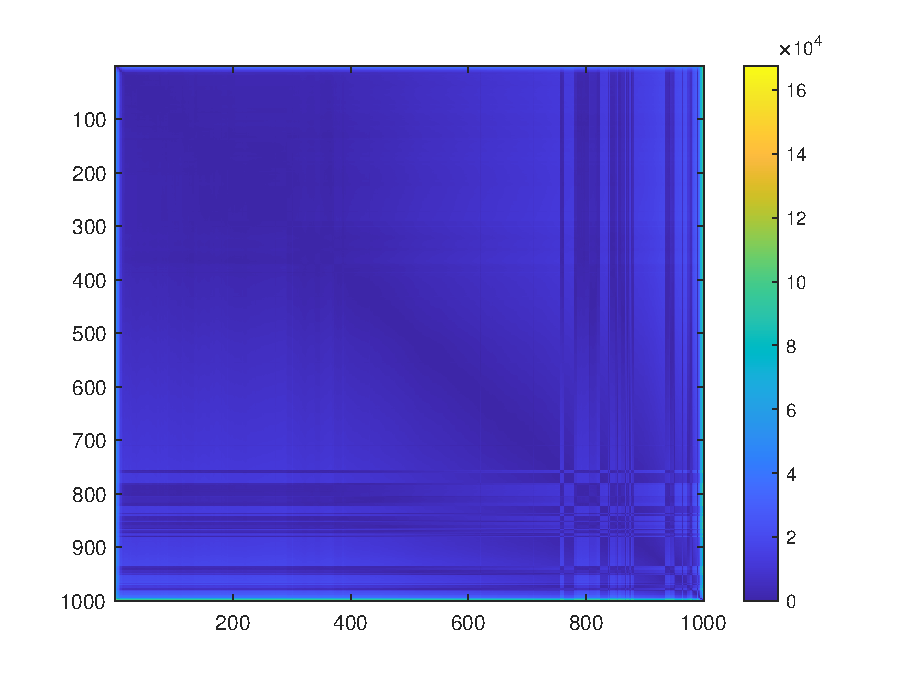
\includegraphics[width=0.85\textwidth]{figuras/vat_time_500.eps}
	\caption{VAT usando 500 épocas de características tipo tiempo continuo.}
	\label{vat: vat_time_500}
\end{figure}
\begin{figure}[H]
	\centering
	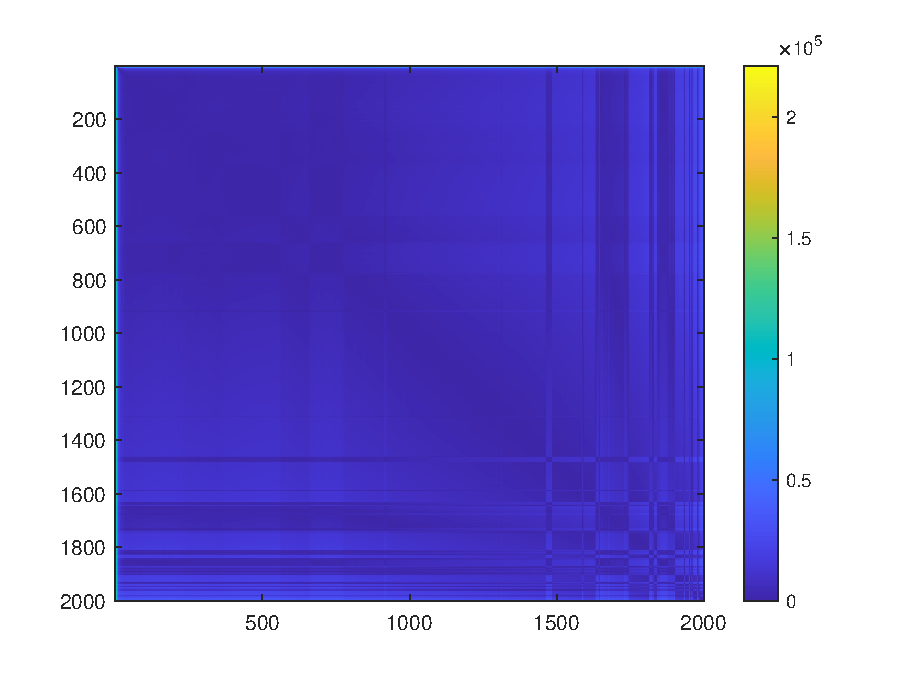
\includegraphics[width=0.85\textwidth]{figuras/vat_time_1000.eps}
	\caption{VAT usando 1000 épocas de características tipo tiempo continuo.}
	\label{vat: vat_time_1000}
\end{figure}
\begin{figure}[H]
	\centering
	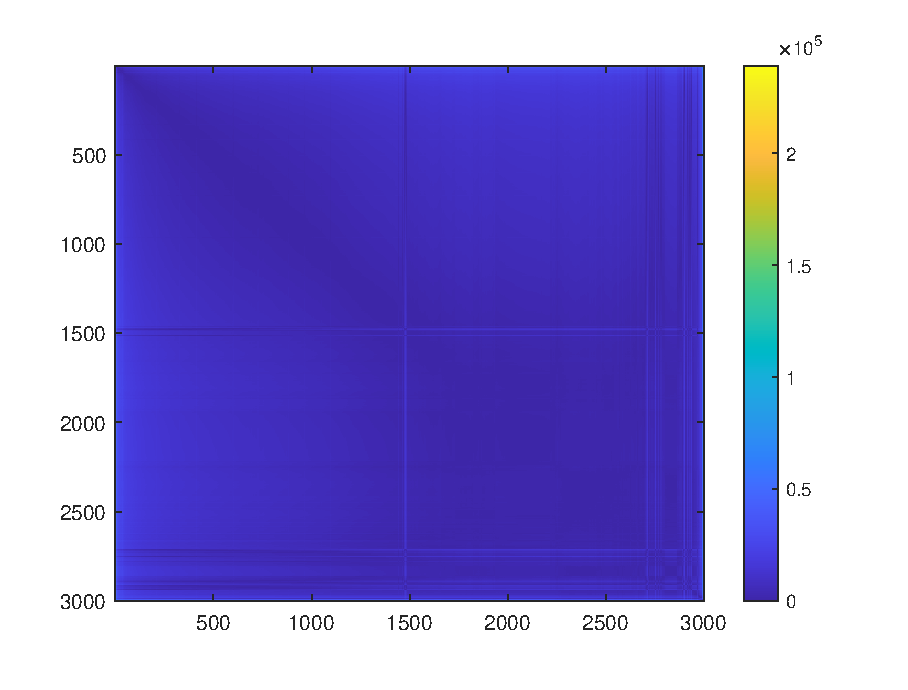
\includegraphics[width=0.85\textwidth]{figuras/vat_time_1500.eps}
	\caption{VAT usando 1500 épocas de características tipo tiempo continuo.}
	\label{vat: vat_time_1500}
\end{figure}
\begin{figure}[H]
	\centering
	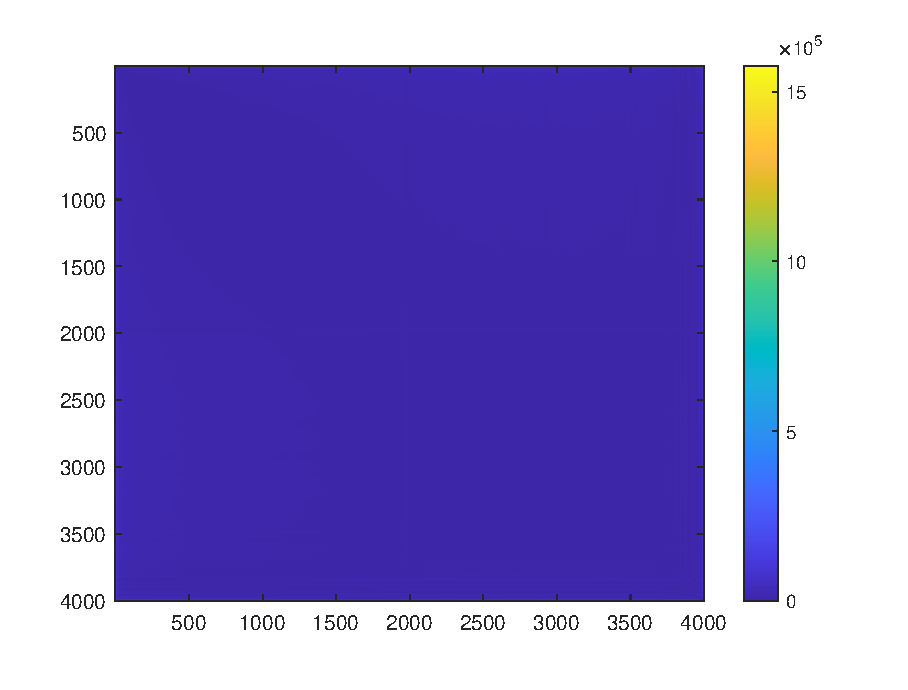
\includegraphics[width=0.85\textwidth]{figuras/vat_time_2000.eps}
	\caption{VAT usando 2000 épocas de características tipo tiempo continuo.}
	\label{vat: vat_time_2000}
\end{figure}
\begin{figure}[H]
	\centering
	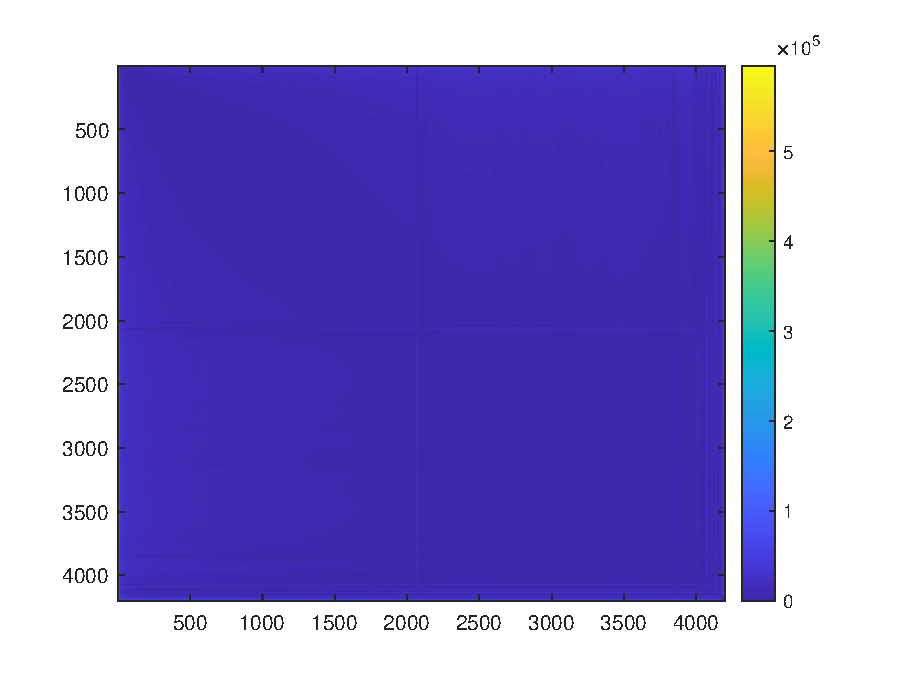
\includegraphics[width=0.85\textwidth]{figuras/vat_time_2100.eps}
	\caption{VAT usando 2100 épocas de características tipo tiempo continuo.}
	\label{vat: vat_time_2100}
\end{figure}
\begin{figure}[H]
	\centering
	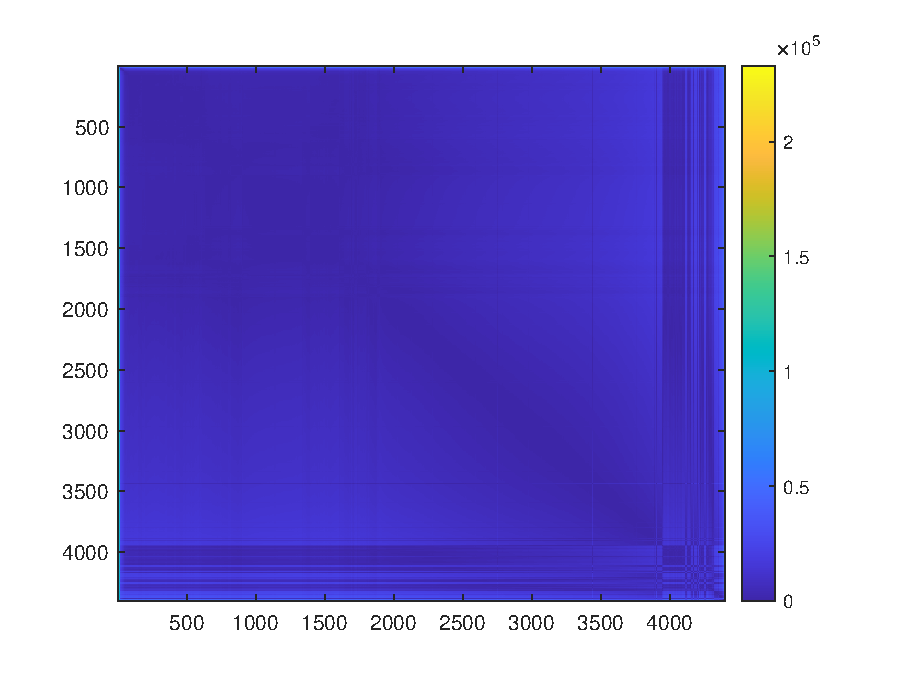
\includegraphics[width=0.85\textwidth]{figuras/vat_time_2200.eps}
	\caption{VAT usando 2200 épocas de características tipo tiempo continuo.}
	\label{vat: vat_time_2200}
\end{figure}
\begin{figure}[H]
	\centering
	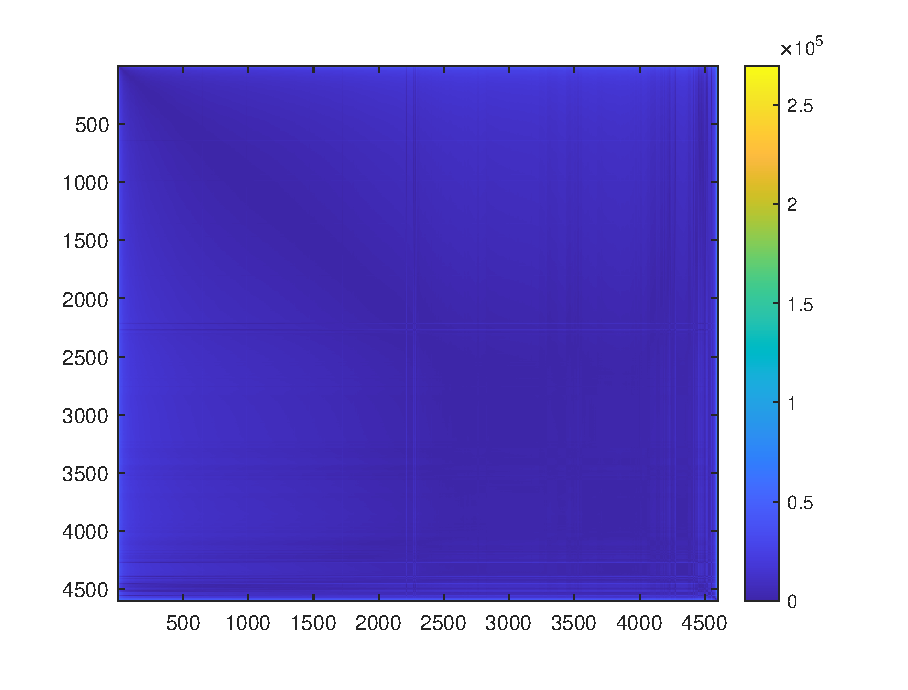
\includegraphics[width=0.85\textwidth]{figuras/vat_time_2300.eps}
	\caption{VAT usando 2300 épocas de características tipo tiempo continuo.}
	\label{vat: vat_time_2300}
\end{figure}


\subsection{VAT características en el dominio de wavelets}
La aplicación del algoritmo VAT a las características extraídas en el dominio de wavelets revela resultados notables en la diferenciación de patrones en las señales bioeléctricas. La representación visual muestra una clara distinción entre dos grupos, evidenciada por la marcada variación de colores. Esta observación sugiere que las características en el dominio de wavelets utilizadas en el análisis poseen una capacidad discriminatoria sobresaliente, permitiendo una separación efectiva entre las señales asociadas a estados sanos y ictales. La nitidez en la identificación de estos grupos mediante VAT en el dominio de wavelets subraya la importancia y relevancia de estas características para el análisis y clasificación de señales bioeléctricas. Estos resultados prometedores proporcionan una base sólida para considerar el dominio de wavelets como un enfoque valioso en la identificación de patrones distintivos en señales bioeléctricas relacionadas con la epilepsia. Para ello observar las Figuras~\ref{vat: vat_wavelets_100} - \ref{vat: vat_wavelets_2300}.

\begin{figure}[H]
	\centering
	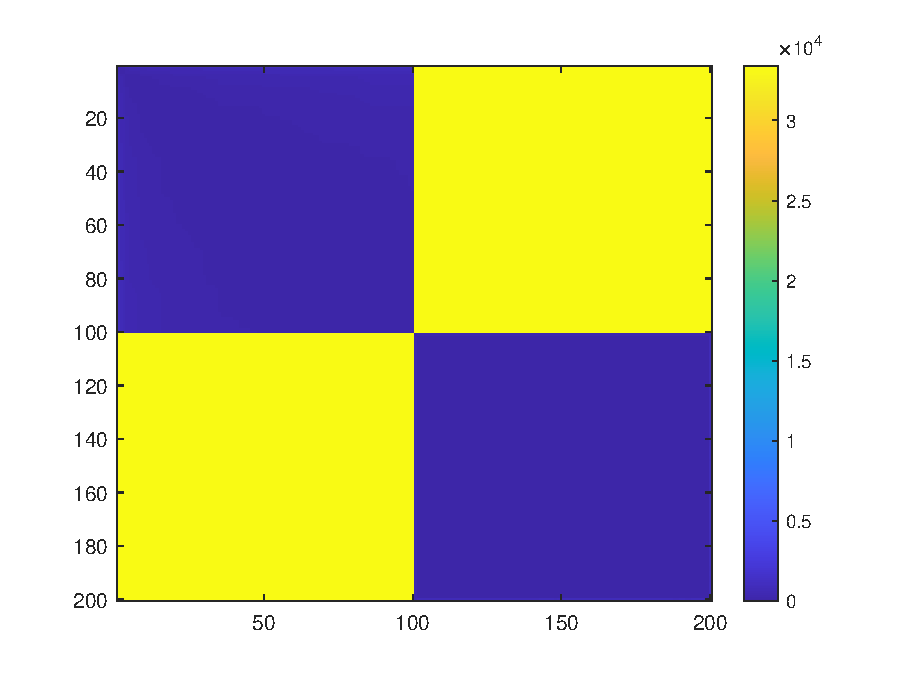
\includegraphics[width=0.85\textwidth]{figuras/vat_wavelets_100.eps}
	\caption{VAT usando 100 épocas de características tipo wavelets.}
	\label{vat: vat_wavelets_100}
\end{figure}
\begin{figure}[H]
	\centering
	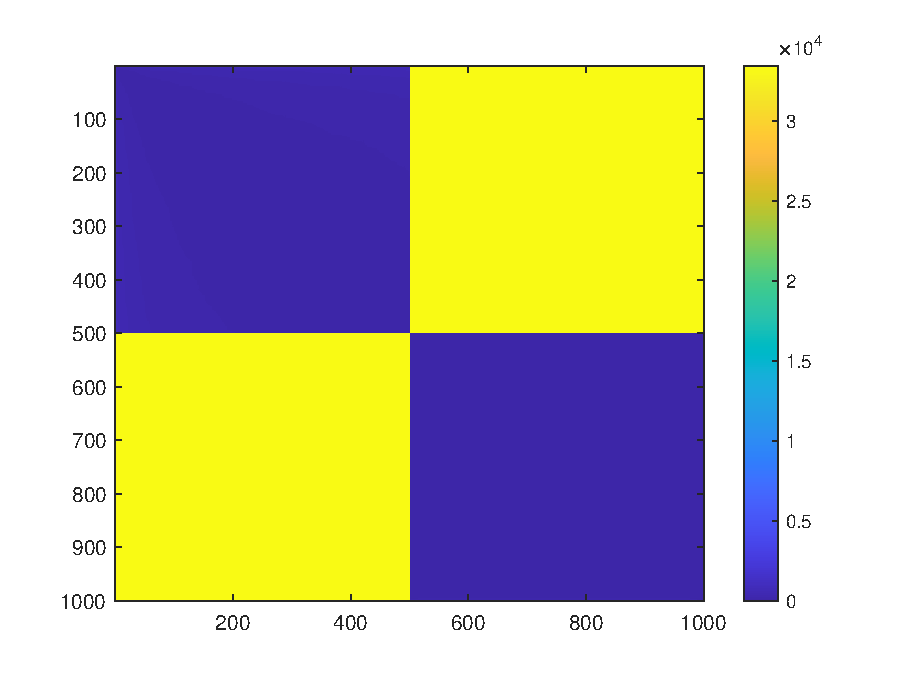
\includegraphics[width=0.85\textwidth]{figuras/vat_wavelets_500.eps}
	\caption{VAT usando 500 épocas de características tipo wavelets.}
	\label{vat: vat_wavelets_500}
\end{figure}
\begin{figure}[H]
	\centering
	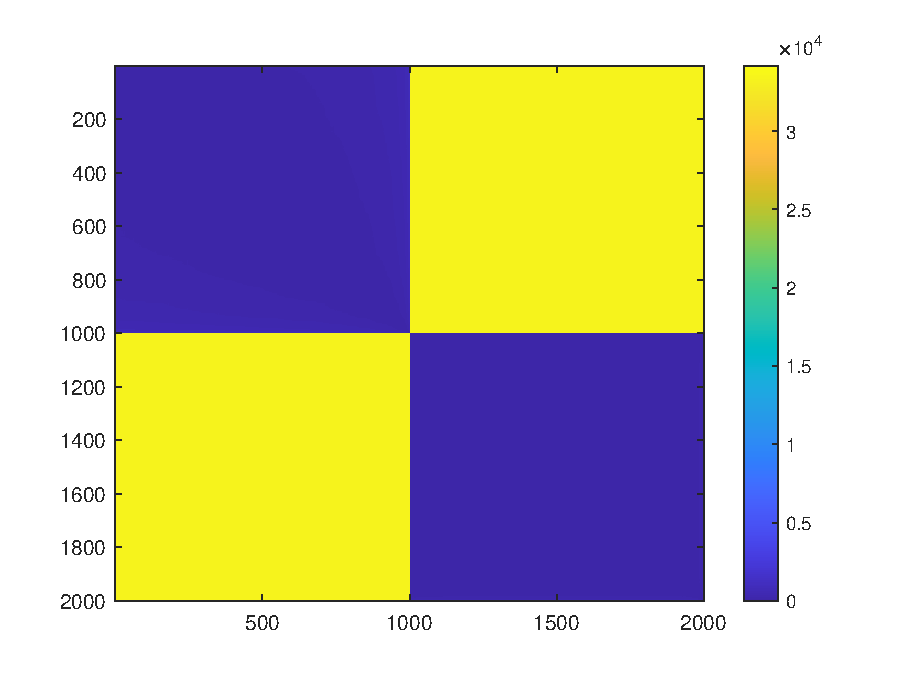
\includegraphics[width=0.85\textwidth]{figuras/vat_wavelets_1000.eps}
	\caption{VAT usando 1000 épocas de características tipo wavelets.}
	\label{vat: vat_wavelets_1000}
\end{figure}
\begin{figure}[H]
	\centering
	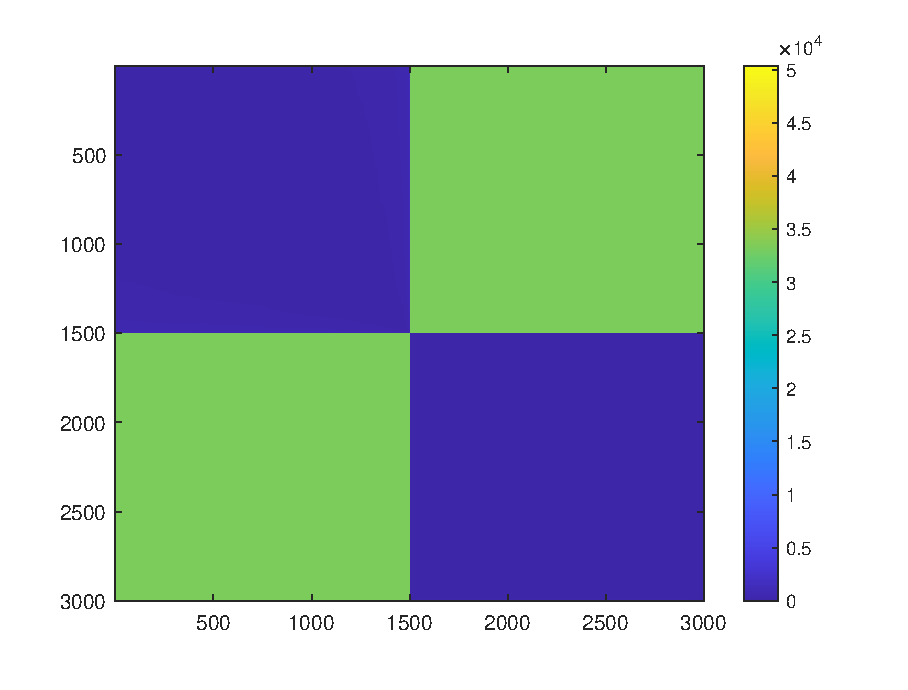
\includegraphics[width=0.85\textwidth]{figuras/vat_wavelets_1500.eps}
	\caption{VAT usando 1500 épocas de características tipo wavelets.}
	\label{vat: vat_wavelets_1500}
\end{figure}
\begin{figure}[H]
	\centering
	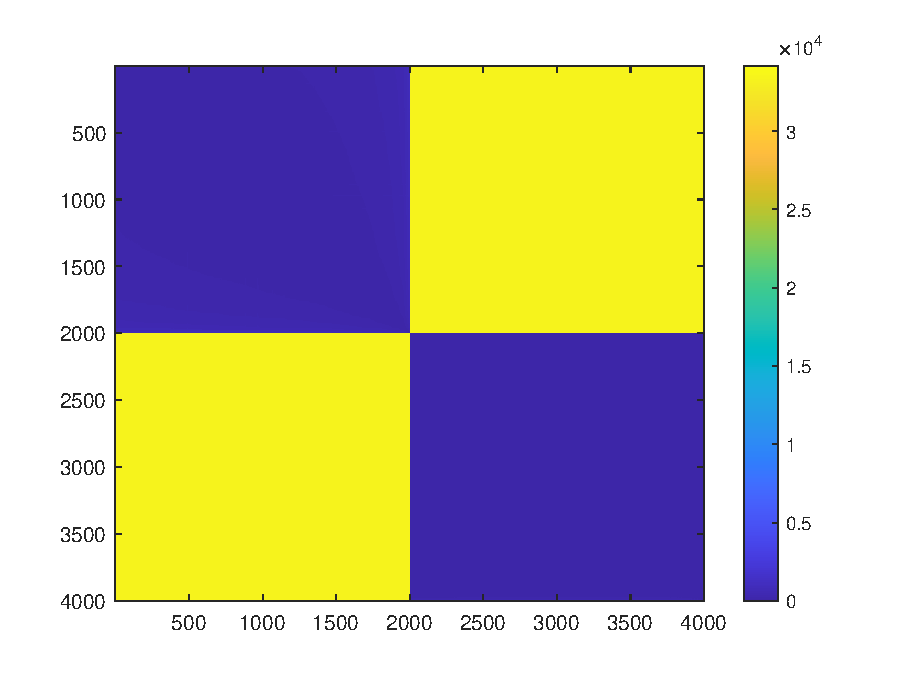
\includegraphics[width=0.85\textwidth]{figuras/vat_wavelets_2000.eps}
	\caption{VAT usando 2000 épocas de características tipo wavelets.}
	\label{vat: vat_wavelets_2000}
\end{figure}
\begin{figure}[H]
	\centering
	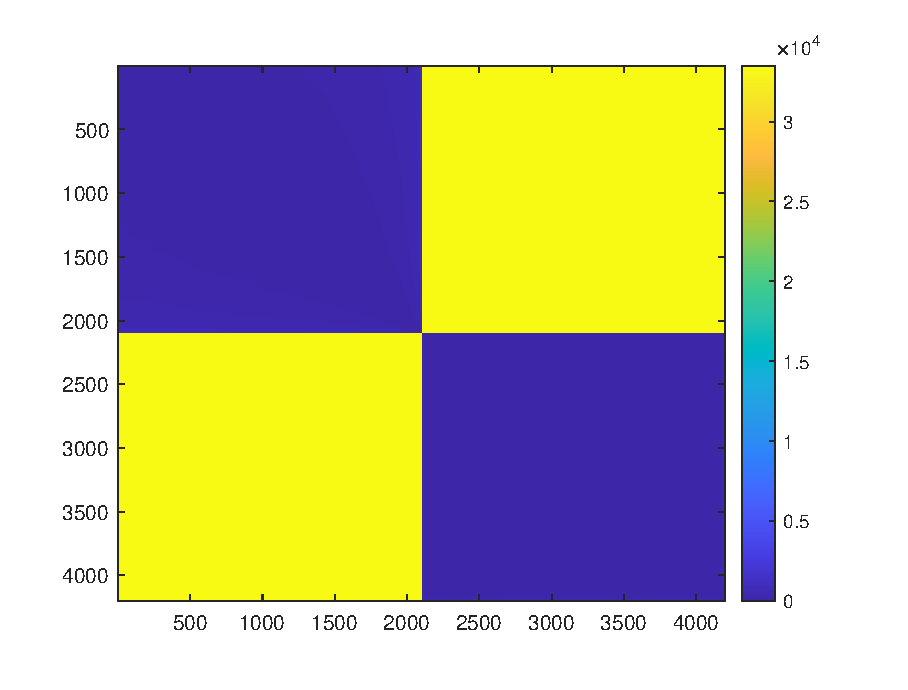
\includegraphics[width=0.85\textwidth]{figuras/vat_wavelets_2100.eps}
	\caption{VAT usando 2100 épocas de características tipo wavelets.}
	\label{vat: vat_wavelets_2100}
\end{figure}
\begin{figure}[H]
	\centering
	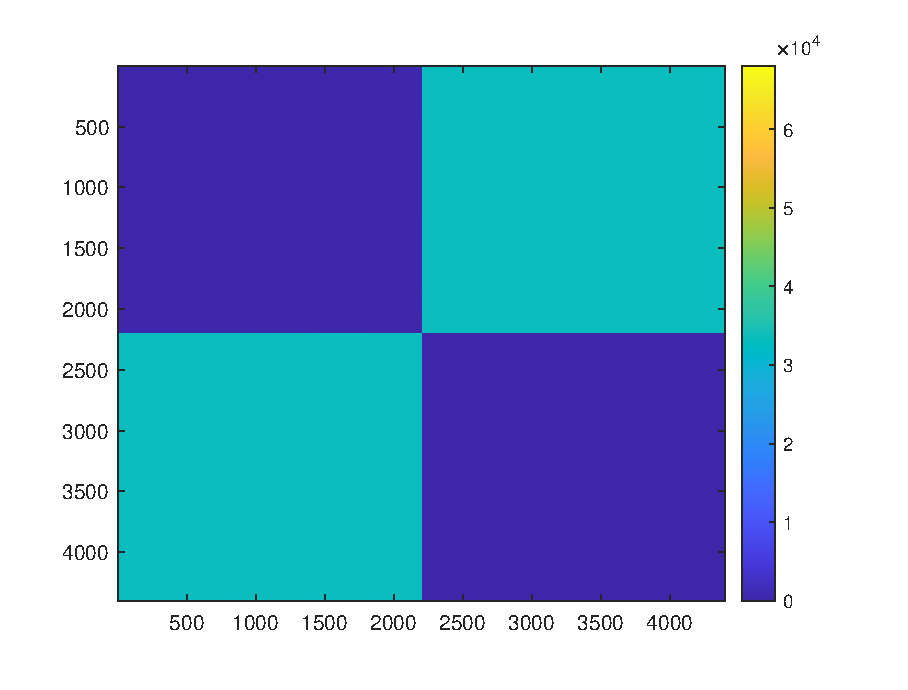
\includegraphics[width=0.85\textwidth]{figuras/vat_wavelets_2200.eps}
	\caption{VAT usando 2200 épocas de características tipo wavelets.}
	\label{vat: vat_wavelets_2200}
\end{figure}
\begin{figure}[H]
	\centering
	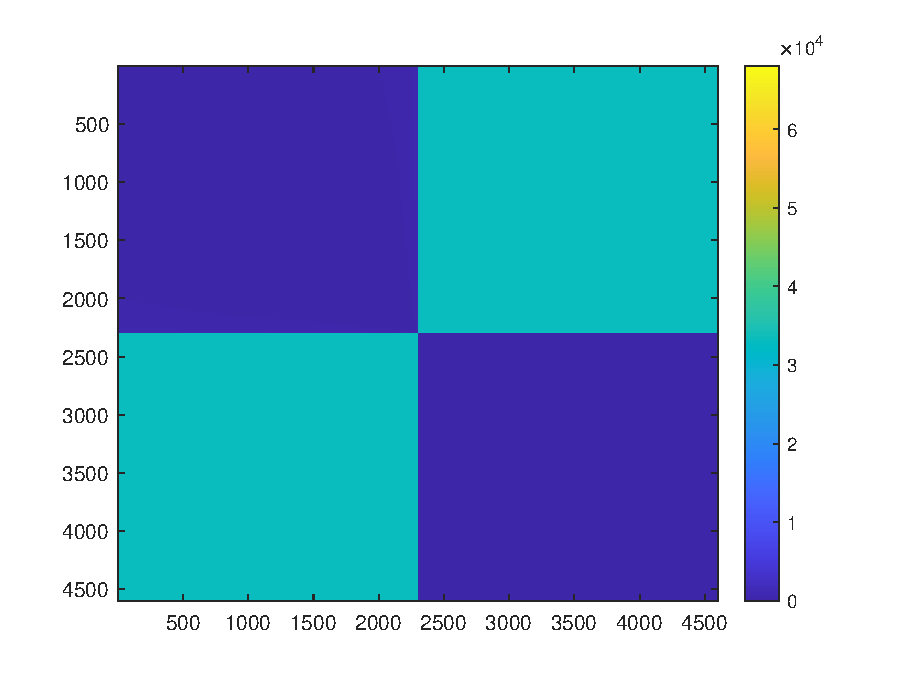
\includegraphics[width=0.85\textwidth]{figuras/vat_wavelets_2300.eps}
	\caption{VAT usando 2300 épocas de características tipo wavelets.}
	\label{vat: vat_wavelets_2300}
\end{figure}

